\documentclass{report}
\usepackage{ucs} 
\usepackage[utf8x]{inputenc} 	
\usepackage[czech]{babel}
\usepackage{pdfpages}
\usepackage{hyperref}
\usepackage{graphicx}
\usepackage{datetime}
\usepackage{titlesec}
\usepackage{interval}
\usepackage{multirow}
\usepackage{tikz-timing}
\usepackage{tikz}
\usepackage{listings}
\usepackage{nextpage}

\graphicspath{ {./Schematics/} }
\newcommand*\wildcard[2][5cm]{\vspace*{2cm}\parbox{#1}{\hrulefill\par#2}}  

\title{TuxMan - FPGA}
\titleformat{\paragraph}
\date{11/4/2019}
\author{Martin Přívozník}

\begin{document}
  \includepdf[page={1}]{FrontPage}
  \newpage
  \pagenumbering{gobble}

 \includepdf[page={3}]{FrontPage}

\newpage
\tableofcontents
\listoffigures
\listoftables

\newpage
\pagenumbering{arabic}

\chapter*{Úvod}
\addcontentsline{toc}{section}{Úvod}
Cílem práce je navrhnout a implementovat číslicový logický obvod realizující arkádovou hru. Číslicový obvod bude umět zpracovat příchozí signál z PS/2 klávesnice, obsluhovat VGA monitor a řídit chod hry. K implementaci mého návrhu využiji přípravek Basys 2 od firmy Digilent s vestavěným FPGA Spartan-E3. Důvodem k využití tohoto přípravku jsou vestavěné porty PS/2 a VGA a dostatečné splnění požadavků pro implementaci. Motivací ke psaní této práce je obsáhlá teorie potřebná pro návrh a implementaci obvodu, jíž se bude zaobírat značná část práce. Výstup této práce nebude tedy pouze funkční arkádová hra, ale také seznámení s problematikou řešení pomocí číslicových obvodů a průvod tím, jak může probíhat návrh komplexnějšího číslicového obvodu vč. implementace na vybrané FPGA.

\chapter{Analýza}
Tato kapitola obsahuje stručný souhrn znalostí a informací potřebných pro následný návrh a implementaci. V sekci~\ref{sec:cislicovynavrh} je vysvětlen číslicový obvod a postup jeho návrhu. V sekci~\ref{sec:fpga} stručně vysvětluji programovatelné hradlové pole a dále vybranou vývojovou desku. Sekce~\ref{sec:rozhrani} se zabývá použitými komunikačními rozhraními, které zajišťují uživatelský vstup a výstup. Na závěr kapitoly, v sekci~\ref{sec:hrapacman} vysvětluji princip a funkčnost hry, jenž je vzorem pro můj návrh.

\section{Číslicový návrh}\label{sec:cislicovynavrh}
V této sekci se věnuji tomu, co je číslicový obvod a jak jej navrhnout jak ve schématu, tak v jazyce popisujícím hardware. V podsekci~\ref{sec:kombinacniobvody} rozeberu logické funkce, prostředky jejich popisu a realizace pomocí logických hradel. Podsekce~\ref{sec:sekvencniobvody}  je zaměřená na návrh sekvenčních obvodů a synchronních sekvenčních automatů (FSM), na což naváže podsekce~\ref{sec:synchronniaasynchronninavrh}, ve které vysvěluji princip hodinových domén a plně sekvenčního návrhu. V podsekci~\ref{sec:jazykvhdl} stručně ukážu, jak převést schéma číslicového obvodu do kódu v jazyce popisujícím hardware (Hardware Description Language, HDL), v mém případě do jazyka Very High Speed Integrated Circuit Hardware Description Language (VHDL).


\subsection{Kombinační obvody}\label{sec:kombinacniobvody}
\subsubsection{Booleovská funkce}
Booleovská funkce je funkce $N$ vstupů a $M$ výstupů nad množinou $\{0, 1\}$. V případě, kdy má funkce více jak jeden výstup, lze ji rozdělit na $M$ funkcí s jedním výstupem. Uvážíme-li Booleovu algebru, platí pro operace sčítání a násobení pravidla uvedená v tabulce~\ref{tab:pravidla}. 
\begin{table}
\centering
\begin{tabular}{ c c c } 
	$a+ b = b + a$ & $a*b = b*a$ & (komutativita) \\
	$a+(b+c) = (a+b) + c$ & $a*(b*c) = (a*b)*c$ & (asociativita) \\
	$a+(b*c) = (a+b) * (a+c)$ & $a*(b+c) = (a*b) + (a*c)$ & (distributivita) \\
	$a+0 = a$ & $a*1 = a$ & (neutralita 0 a 1) \\
	$a + \overline{a} = 1$ & $a * \overline{a} = 0$ & (vlastnosti negace) \\
\end{tabular}
    \caption{Axiomy a vztahy Booleovy algebry.\cite{boole1854investigation}}
    \label{tab:pravidla}
\end{table}
Operace se dvěma vstupními hodnotami nazýváme binární operace. Některé binární operace, přestože často používají stejná značení + a * jako v algebře reálných čísel, mají v Booleově algebře stejnou prioritu a jiný význam (žádná operace nemá přednost)~\cite{kubatova}. Pro logický součet a logický součin platí základní pravidla v tabulce~\ref{tab:pravidlaboolalgebry}.
\begin{table}
\centering
\begin{tabular}{ c c c } 
	de Morgan & $\overline{(a+b)} = \overline{a} * \overline{b}$ & $\overline{(a*b)} = \overline{a} + \overline{b}$ \\
	idempotence & $a + a = a$ & $a * a = a$ \\
\end{tabular}
    \caption{Základní pravidla Booleovy algebry.\cite{kubatova}}
    \label{tab:pravidlaboolalgebry}
\end{table}
Příkladem reprezentace Booleovské funkce je pravdivostní tabulka~\ref{tab:andtable}, kde $in_1$ a $in_2$ jsou vstupní hodnoty a $out$ je výstupní hodnota. 
\begin{table}
\centering
\begin{tabular}{ |c c|c| } 
   	\hline
	$in_1$ & $in_2$ & $out$ \\
	\hline
	$0$ & $0$ & $f(0,0)$ \\
	$0$ & $1$ & $f(0,1)$ \\
	$1$ & $0$ & $f(1,0)$ \\
	$1$ & $1$ & $f(1,1)$ \\
   	\hline
\end{tabular}
    \caption{Pravdivostní tabulka.}
    \label{tab:andtable}
\end{table}
Pravdivostní tabulka obsahuje vždy $N^2$ řádků, aby reprezentovala výstupní hodnotu pro všechny možné kombinace vstupních hodnot. Další možností je Booleovská formule~.\cite{kubatova}. K vyjádření formule a k popisu booleovské funkce používáme nejčastěji základní funkce uvedené v tabulce~\ref{tab:logickefunkce}
\begin{table}
\centering
\begin{tabular}{ |c|c|c| } 
   	\hline
	Název & Pravdivostní tabulka & Formule \\
   	\hline
	AND (logický součin) & \begin{tabular}{ |c c|c| } 
	   	\hline
		$in_1$ & $in_2$ & $out$ \\
	   	\hline
		$0$ & $0$ & $0$ \\
		$0$ & $1$ & $0$ \\
		$1$ & $0$ & $0$ \\
		$1$ & $1$ & $1$ \\
	   	\hline
	\end{tabular} & $out = in_1*in_2$ \\
   	\hline
	NAND (negovaný logický součin) & \begin{tabular}{ |c c|c| } 
	   	\hline
		$in_1$ & $in_2$ & $out$ \\
	   	\hline
		$0$ & $0$ & $1$ \\
		$0$ & $1$ & $1$ \\
		$1$ & $0$ & $1$ \\
		$1$ & $1$ & $0$ \\
	   	\hline
	\end{tabular} & $out = \overline{in_1*in_2}$ \\
	\hline
	OR (logický součet) & \begin{tabular}{ |c c|c| } 
	   	\hline
		$in_1$ & $in_2$ & $out$ \\
	   	\hline
		$0$ & $0$ & $0$ \\
		$0$ & $1$ & $1$ \\
		$1$ & $0$ & $1$ \\
		$1$ & $1$ & $1$ \\
	   	\hline
	\end{tabular} & $out = in_1+in_2$ \\
	\hline
	NOR (negovaný logický součet) & \begin{tabular}{ |c c|c| } 
	   	\hline
		$in_1$ & $in_2$ & $out$ \\
	   	\hline
		$0$ & $0$ & $1$ \\
		$0$ & $1$ & $0$ \\
		$1$ & $0$ & $0$ \\
		$1$ & $1$ & $0$ \\
	   	\hline
	\end{tabular} & $out = \overline{in_1+in_2}$ \\
	\hline
	NOT (logická negace) & \begin{tabular}{ |c|c| } 
	   	\hline
		$in_1$ & $out$ \\
	   	\hline
		$0$ & $1$ \\
		$1$ & $0$\\
	   	\hline
	\end{tabular} & $out = \overline{in_1}$ \\
	\hline
	BUFFER (opakovač) & \begin{tabular}{ |c|c| } 
	   	\hline
		$in_1$ & $out$ \\
	   	\hline
		$0$ & $0$ \\
		$1$ & $1$\\
	   	\hline
	\end{tabular} & $out = in_1$ \\
	\hline
	XOR (nonekvivalence) & \begin{tabular}{ |c c|c| } 
	   	\hline
		$in_1$ & $in_2$ & $out$ \\
	   	\hline
		$0$ & $0$ & $0$ \\
		$0$ & $1$ & $1$ \\
		$1$ & $0$ & $1$ \\
		$1$ & $1$ & $0$ \\
	   	\hline
	\end{tabular} & $out = in_1 \oplus in_2$ \\
	\hline
	XNOR (ekvivalence) & \begin{tabular}{ |c c|c| } 
	   	\hline
		$in_1$ & $in_2$ & $out$ \\
	   	\hline
		$0$ & $0$ & $1$ \\
		$0$ & $1$ & $0$ \\
		$1$ & $0$ & $0$ \\
		$1$ & $1$ & $1$ \\
	   	\hline
	\end{tabular} & $out =\overline{in_1 \oplus in_2}$ \\
   	\hline
\end{tabular}
    \caption{Tabulka nejpoužívanějších základních logických funkcí.}
    \label{tab:logickefunkce}
\end{table}
\subsubsection{Kombinační obvod}
Kombinační logický obvod, je takový obvod, ve kterém jsou výstupní hodnoty dány pouze aktuální kombinací vstupních proměnných. Neobsahuje žádnou paměť předchozích stavů. Jedinou vyjímkou je krátký časový interval, za který logický člen (AND, NAND, OR, NOR ...) vyhodnotí výstup na základě vstupních hodnot. Tento časový interval může být zanedbatelný v případě krátkých datových cest. V případě dlouhé datové cesty může být potřeba na tento časový interval brát zřetel a zvážit optimálnější řešení. \par
Platí, že u číslicových obvodů každá proměnná v operaci nabývá hodnotu jednoho tzv. bitu. Bit je základní jednotkou dat a může nabývat hodnot $0$, nebo $1$. Reprezentací číslicového obvodu je schéma číslicového obvodu, kde každá z funkcí je reprezentována tzv. schématickou značkou. Schématické značky mohou být různé, dokud z nich jasně vyplívá, jakou funkci zastupují. Schématické značky jsou propojené signály, které představují jednotlivé bity. Pro minimalizaci je možné několik signálů (bitů) zakreslit jediným konektorem, pokud je označený počtem bitů, které reprezentuje. Nejčastěji používané normy značení jsou evropská a americká. Příklady schéma\-tických značek pro nejpoužívanější logické funkce jsou uvedené v tabulce~\ref{tab:functionschemes}. 
\begin{table}
\centering
\begin{tabular}{ c c } 
	AND & \raisebox{-0.4\height}{\includegraphics[scale=0.6]{/Gates/AND.png}} \\
	NAND & \raisebox{-0.4\height}{\includegraphics[scale=0.6]{/Gates/NAND.png}} \\
	OR & \raisebox{-0.4\height}{\includegraphics[scale=0.6]{/Gates/OR.png}} \\
	NOR & \raisebox{-0.4\height}{\includegraphics[scale=0.6]{/Gates/NOR.png}} \\
	NOT & \raisebox{-0.4\height}{\includegraphics[scale=0.6]{/Gates/NOT.png}} \\
	BUFFER & \raisebox{-0.4\height}{\includegraphics[scale=0.6]{/Gates/BUFFER.png}} \\
	XOR & \raisebox{-0.4\height}{\includegraphics[scale=0.6]{/Gates/XOR.png}} \\
	XNOR & \raisebox{-0.4\height}{\includegraphics[scale=0.6]{/Gates/XNOR.png}} \\
\end{tabular}
    \caption{Schématické značky některých nejpouživanějších základních logických funkcí (americká norma ANSI).}
    \label{tab:functionschemes}
\end{table}
Pro usnad\-nění práce můžeme využívat logických bloků, které plní danou funkci. Opět platí, že ze značení logických bloků ve schématu musí plně vyplívat, jakou funkci zastupují. Logický blok, který má definovanou funkci může být použit schématu. Při návrhu číslicových obvodů využíváme hierarchie, kde jsou pro každý logický blok popsány vstupy i výstupy a v případě, kdy se nejedná o základní logické bloky, tak je popsána i funkce (formule, pravdivostní tabulka, nebo schéma bloku) a vhodně přiřazena ke schématu. Jedním ze základních logických bloků je poloviční sčítačka, viz obrázek~\ref{fig:halfadder}.
\begin{figure}
\centering
\includegraphics[width=0.9\columnwidth]{/LogicalBlocks/HalfAdder.png}
\caption{Schéma poloviční sčítačky a příklad jejího značení ve schématu.}
\label{fig:halfadder}
\end{figure}
 Poloviční sčítačka umí sečíst dvě jednobitová čísla a vygenerovat bit do vyššího řádu (carry) podle pravdivostní tabulky~\ref{tab:halfaddertab}.
\begin{table}
\centering
 \begin{tabular}{ |c c|c c| } 
   	\hline
	$A$ & $B$ & $C$ & $\sum$ \\
   	\hline
	$0$ & $0$ & $0$ & $0$ \\
	$0$ & $1$ & $0$ & $1$\\
	$1$ & $0$ & $0$ & $1$\\
	$1$ & $1$ & $1$ & $0$\\
   	\hline
\end{tabular}
	\caption{Pravdivostní tabulka poloviční sčítačky.}
	\label{tab:halfaddertab}
\end{table}
Zřetězením dvou polovičních sčítaček a přenesením pomocí funkce OR získáme poté kompletní sčítačku, viz obrázek~\ref{fig:fulladder}.\cite{kubatova}
\begin{figure}
\centering
\includegraphics[width=0.9\columnwidth]{/LogicalBlocks/FullAdder.pdf}
\caption{Schéma kompletní sčítačky a příklad jejího značení ve schématu.}
\label{fig:fulladder}
\end{figure}
Kompletní sčítačka umí sečíst jednobitová čísla, vygenerovat bit do vyššího řádu a přijmout bit z nižšího, sčítá tedy tři bity. Sčítá počet jedniček na vstupech. \par
Pro porovnávání dvou hodnot a vyhodnocení jejich nerovnosti používáme tzv. komparátor, viz obrázek~\ref{fig:comparator}. 
\begin{figure}
\centering
\includegraphics[width=0.9\columnwidth]{/LogicalBlocks/Comparator.pdf}
\caption{Schéma komparátoru a příklad jeho značení ve schématu.}
\label{fig:comparator}
\end{figure}
Dalším důležitým základním logickým blokem je multiplexor, viz obrázek~\ref{fig:mux}.
\begin{figure}
\centering
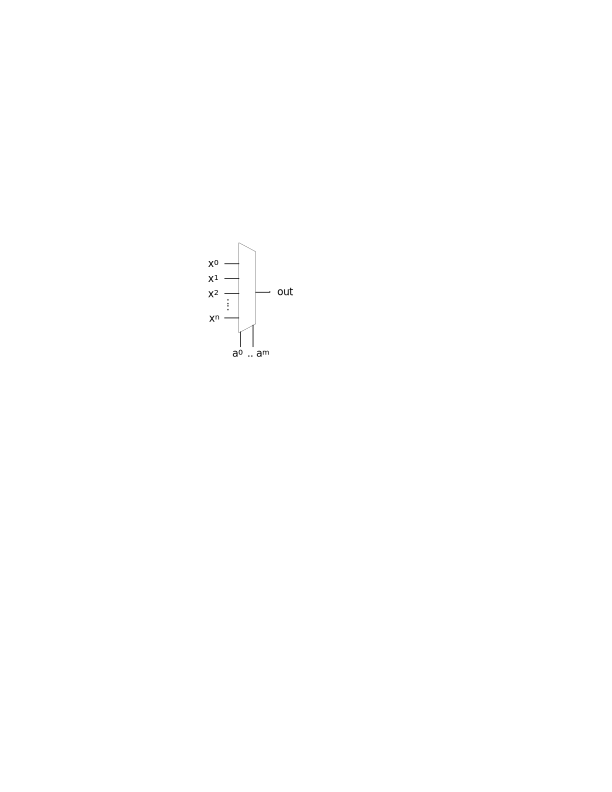
\includegraphics[width=0.6\columnwidth]{/LogicalBlocks/Mux.pdf}
\caption{Schématická značka multiplexoru.}
\label{fig:mux}
\end{figure}
Multiplexor na základě řídícího vstupu/řídících vstupů ($a$) přivádí na výstup ($out$) jeden ze vstupních signálů ($x$). \par
Číslicový obvod lze realizovat například z integrovaných obvodů, v nichž bývají hradla realizována z několika tranzistorů. Logické hodnoty představuje napětí přivedené na obvod. Logická $1$ bývá reprezentována  napětím kladným a logická $0$ napětím nulovým.

\subsection{Sekvenční obvody}\label{sec:sekvencniobvody}
\subsubsection{Sekvenční logický obvod}
Sekvenční logický obvod je takový obvod, ve kterém výstupní hodnoty nejsou dány pouze aktuální kombinací vstupních proměnných, ale zároveň jeho vnitřním stavem. Sekvenční obvod si tedy musí zapamatovat předchozí hodnoty pomocí paměti, která bývá realizována pomocí zpětné vazby~\cite{kubatova}. Sekvenční obvod se dělí na dvě části - kombinační a paměťovou, kde paměťová část je tvořena logickým obvodem, ve kterém bývá zavedena zpětná vazba a kombinační část bývá tvořena kombinačním obvodem. Obecné schéma sekvenčního obvodu je na obrázku~\ref{fig:seqcircuit}. \par
\begin{figure}
\centering
\includegraphics[width=0.9\columnwidth]{/LogicalBlocks/sqcircuit.pdf}
\caption{Huffmanův model sekvenčního obvodu.}
\label{fig:seqcircuit}
\end{figure}
Příkladem logického obvodu se zpětnou vazbou může být tzv. RS klopný obvod, viz obrázek~\ref{fig:rsko}.
\begin{figure}
\centering
\includegraphics[width=0.9\columnwidth]{/LogicalBlocks/RSKO.pdf}
\caption{Schéma RS klopného obvodu s využitím logických hradel NOR.}
\label{fig:rsko}
\end{figure}
RS klopný obvod překlápí mezi dvěma mezními hodnotami. Pravdivostní tabulka RS klopného obvodu se může dělit na tři části - zakázaný stav (ZS), překlápěcí část a paměť, viz tabulka~\ref{tab:rskotab}.
\begin{table}
\centering
 \begin{tabular}{ |c c|c c| } 
   	\hline
	$A$ & $B$ & $Q$ & $Q'$ \\
   	\hline
	$0$ & $0$ & \multicolumn{2}{c|}{Z.S.} \\
	$0$ & $1$ & $0$ & $1$\\
	$1$ & $0$ & $1$ & $0$\\
	$1$ & $1$ & \multicolumn{2}{c|}{Paměť}\\
   	\hline
\end{tabular}
	\caption{Pravdivostní tabulka RS klopného obvodu s využitím NOR.}
	\label{tab:rskotab}
\end{table}
Pokud se tedy změní vstupní hodnoty z $[0,1]$, nebo $[1,0]$ na $[1,1]$, na výstupu bude předchozí hodnota, dokud neproběhne další změna vstupních hodnot. Jedná se tedy o tzv. hladinový klopný obvod (angl. latch). Častěji využívaným klopným obvodem je tzv. D klopný obvod, viz obrázek~\ref{fig:dko}.
\begin{figure}
\centering
\includegraphics[width=0.9\columnwidth]{/LogicalBlocks/DKO.pdf}
\caption{Schéma D klopného obvodu.}
\label{fig:dko}
\end{figure}
Výhodou D klopného obvodu je fakt, že narozdíl od RS klopného obvodu nemá zakázaný stav, viz pravdivostní tabulka~\ref{tab:dkotab}.
\begin{table}
\centering
 \begin{tabular}{ |c c|c c| } 
   	\hline
	$T$ & $D$ & $Q$ & $Q'$ \\
   	\hline
	\texttiming{LH} & $x$ & $x$ & $\overline{x}$\\
	\multicolumn{2}{|c|}{Jinak} & \multicolumn{2}{|c|}{Paměť}\\
   	\hline
\end{tabular}
	\caption{Pravdivostní tabulka D klopného obvodu.}
	\label{tab:dkotab}
\end{table}
Signál $T$ u D klopného obvodu se dá považovat za tzv. povolovací signál. Při náběžné hraně na $T$  (změna stavu z logické $0$ na logickou $1$) se na výstup $Q$ zapíše aktuální hodnota na signálu $D$. V tomto případě se tedy jedná o hranový klopný obvod. Příklad značení D klopného obvodu je na obrázku~\ref{fig:dblock}.
\begin{figure}
\centering
\includegraphics[width=0.4\columnwidth]{/LogicalBlocks/DBlock.pdf}
\caption{Příklad značení D klopného obvodu ve schématu.}
\label{fig:dblock}
\end{figure}
Vstupní signál označený trojúhelníkem je signál T. Trojúhelník značí, že obvod mění výstupní hodnotu v reakci na náběžnou hranu. Tento vstup se jinak nazývá hodinovým vstupem. Pokud má číslicový obvod takový vstup jedná se o sekvenční obvod. V případě hladinového obvodu by ve značení mohl být místo trojúhelníku čtverec. \par
Hodnoty na signálech se dají popsat tzv. časovým diagramem. Časový diagram popisuje, jaké logické hodnoty nabývá daný signál v jaký čas. Příklad časového diagramu je na obrázku~\ref{fig:dkotd}.
\begin{figure}
\centering
\includegraphics[width=0.6\columnwidth]{/TimeDiagrams/DFlipFlop.pdf}
\caption{Časový diagram D klopného obvodu.}
\label{fig:dkotd}
\end{figure}
\par
Příkladem sekvenčního logického bloku je čítač. Čítač je takový sekvenční logický obvod, který uchovává v ,,paměti" informaci o tom, kolikrát zaznamenal změnu stavu (dle návrhu náběžnou, nebo sestupnou hrana) na hodinovém signálu. Příklad schématu čítače je na obrázku~\ref{fig:counter}.
\begin{figure}
\centering
\includegraphics[width=0.9\columnwidth]{/LogicalBlocks/Counter.pdf}
\caption{Příklad schématu dvoubitového čítače reagujícího na náběžnou hranu.}
\label{fig:counter}
\end{figure}
Může být ve schématu značen, jako na obrázku~\ref{fig:counterbox}.
\begin{figure}
\centering
\includegraphics[width=0.4\columnwidth]{/LogicalBlocks/Counterbox.pdf}
\caption{Příklad schématické značky dvoubitového čítače reagujícího na náběžnou hranu.}
\label{fig:counterbox}
\end{figure}
\subsubsection{Konečný stavový automat}
Konečný stavový automat (angl. Finite State Machine - FSM) M je šestice M=(Q, T, D, $\delta$, $\lambda$, $q_0$), kde~\cite{jazykyapreklady}:
\begin{itemize}
  \item Q je konečná množina vnitřních stavů
  \item T je konečná množina vstupních symbolů (signálů)
  \item D je konečná množina výstupních symbolů (signálů)
  \item $\delta$ je zobrazení z Q x T do Q (stav x vstup do stav) nazývané přechodová funkce
  \item $\lambda$ je zobrazení z Q x T do D (Mealy, ze stavu a vstupu do výstupu) nebo Q do D (Moore, jen ze stavu do výstupu)
  \item $q_0$ je počáteční stav
\end{itemize}
Má definované stavy, mezi kterými za daných podmínek přepíná a mění svůj výstup. FSM provádí vždy právě jeden přechod s každou náběžnou hranou hodin. Musí popisovat přechodovou funkci (podmínky pro změnu stavu a do kterého), výstupní funkci (jaký signál v danou chvíli udává na výstup) a dále musí mít definovaný počátečný stav. Příklad stavového diagramu FSM je na obrázku~\ref{fig:fsmexample}, kde $a, b, c$ jsou podmínky pro změnu stavu a $q1, q2, q3$ jsou stavy FSM. Počáteční stav je značen šipkou, která nevychází z žádného stavu, v tomto případě $q1$.
\begin{figure}
\begin{center}
\begin{tikzpicture}[scale=0.2]
\tikzstyle{every node}+=[inner sep=0pt]
\draw [black] (22.4,-28.4) circle (3);
\draw (22.4,-28.4) node {$q1$};
\draw [black] (39.9,-28.4) circle (3);
\draw (39.9,-28.4) node {$q2$};
\draw [black] (57.8,-28.4) circle (3);
\draw (57.8,-28.4) node {$q3$};
\draw [black] (25.4,-28.4) -- (36.9,-28.4);
\fill [black] (36.9,-28.4) -- (36.1,-27.9) -- (36.1,-28.9);
\draw (31.15,-27.9) node [above] {$a$};
\draw [black] (42.9,-28.4) -- (54.8,-28.4);
\fill [black] (54.8,-28.4) -- (54,-27.9) -- (54,-28.9);
\draw (48.85,-27.9) node [above] {$b$};
\draw [black] (55.587,-30.423) arc (-51.04855:-128.95145:24.636);
\fill [black] (24.61,-30.42) -- (24.92,-31.31) -- (25.55,-30.54);
\draw (40.1,-36.4) node [below] {$c$};
\draw [black] (15.5,-28.4) -- (19.4,-28.4);
\fill [black] (19.4,-28.4) -- (18.6,-27.9) -- (18.6,-28.9);
\end{tikzpicture}
\end{center}
\caption{Příklad stavového diagramu konečného stavového automatu.}
\label{fig:fsmexample}
\end{figure}
Rozeznáváme dva typy FSM na základě definičního oboru výstupní funkce~\cite{kubatova, jazykyapreklady}. Prvním typem je typ Mealy (angl. často input-based), který mění svůj výstup na základě aktuálního stavu a změn na vstupních signálech. Druhý je typ Moore (angl. často state-based), jehož výstupní funkce je závislá pouze na aktuálním stavu (každý stav má definovaný výstup). Příkladem stavového diagramu čítače modulo 4 s povolujícím vstupem je obrázek~\ref{fig:counterfsm}
\begin{figure}
\begin{center}
\begin{tikzpicture}[scale=0.2]
\tikzstyle{every node}+=[inner sep=0pt]
\draw [black] (30.5,-22.2) circle (3);
\draw (30.5,-22.2) node {$q0/00$};
\draw [black] (53.2,-22.2) circle (3);
\draw (53.2,-22.2) node {$q1/01$};
\draw [black] (53.2,-41.8) circle (3);
\draw (53.2,-41.8) node {$q2/10$};
\draw [black] (30.5,-41.8) circle (3);
\draw (30.5,-41.8) node {$q3/11$};
\draw [black] (31.931,-19.572) arc (144.37918:35.62082:12.202);
\fill [black] (51.77,-19.57) -- (51.71,-18.63) -- (50.9,-19.21);
\draw (41.85,-13.98) node [above] {$CE\mbox{ }=\mbox{ }1$};
\draw [black] (55.984,-23.288) arc (60.10415:-60.10415:10.049);
\fill [black] (55.98,-40.71) -- (56.93,-40.75) -- (56.43,-39.88);
\draw (61.52,-32) node [right] {$CE\mbox{ }=\mbox{ }1$};
\draw [black] (19.5,-22.2) -- (27.5,-22.2);
\draw (19,-22.2) node [left] {$reset$};
\fill [black] (27.5,-22.2) -- (26.7,-21.7) -- (26.7,-22.7);
\draw [black] (51.63,-44.348) arc (-38.52063:-141.47937:12.5);
\fill [black] (32.07,-44.35) -- (32.18,-45.29) -- (32.96,-44.66);
\draw (41.85,-49.56) node [below] {$CE\mbox{ }=\mbox{ }1$};
\draw [black] (27.936,-40.262) arc (-129.04509:-230.95491:10.637);
\fill [black] (27.94,-23.74) -- (27,-23.85) -- (27.63,-24.63);
\draw (23.5,-32) node [left] {$CE\mbox{ }=\mbox{ }1$};
\draw [black] (33.287,-23.278) arc (96.59379:-191.40621:2.25);
\draw (38.43,-27.66) node [below] {$CE\mbox{ }=\mbox{ }0$};
\fill [black] (31.34,-25.07) -- (30.94,-25.92) -- (31.93,-25.81);
\draw [black] (54.87,-19.722) arc (173.74488:-114.25512:2.25);
\draw (59.72,-17.63) node [right] {$CE\mbox{ }=\mbox{ }0$};
\fill [black] (56.18,-22.02) -- (56.92,-22.6) -- (57.03,-21.61);
\draw [black] (55.834,-43.212) arc (89.53768:-198.46232:2.25);
\draw (60.47,-47.79) node [below] {$CE\mbox{ }=\mbox{ }0$};
\fill [black] (53.68,-44.75) -- (53.17,-45.55) -- (54.17,-45.55);
\draw [black] (29.391,-44.575) arc (5.94318:-282.05682:2.25);
\draw (24.94,-47.77) node [left] {$CE\mbox{ }=\mbox{ }0$};
\fill [black] (27.62,-42.61) -- (26.78,-42.19) -- (26.88,-43.19);
\end{tikzpicture}
\end{center}
\caption{Příklad stavového diagramu (typ Moore) čítače modulo 4 se vstupem count enable.}
\label{fig:counterfsm}
\end{figure}

\subsection{Synchronní návrh}\label{sec:synchronniaasynchronninavrh}
\subsubsection{Pravidla návrhu synchronního obvodu}
Synchronní obvod je takový obvod, ve kterém všechny sekvenční části obvodu mají na svůj hodinový vstup přivedený stejný signál, aby měnily svůj stav ve stejný čas. Tento signál můžeme nazývat společné hodiny. Společné hodiny mění svůj stav na dané frekvenci (nejčastěji dle krystalu v obvodu). Část obvodu se společným hodinovým signálem nazýváme hodinovou doménou~\cite{hodinovedomeny}. Pro návrh synchronního obvodu platí několik pravidel, které je nutné dodržet pro zajištění správné funkčnosti. Společné hodiny nesmí být hradlované (signál musí být přiveden přímo k hodinovým vstupům sekvenčních obvodů). V případě hradlování společných hodin může docházet k zákmitům a časovým rezervám v jednotlivých částech obvodu. Dále je nutné, aby obvod obsahoval synchronní reset. Po synchronním resetu obvodu změní stav celý obvod společně a nedojde k časovým nesrovnalostem~\cite{hodinovedomeny}. \par
Při návrhu se nemusí vždy pracovat pouze s jednou hodinovou doménou. Univerzální řešení přechodu mezi hodinovými doménami je dvoubranové FIFO se dvěma hodinovými vstupy.Pro zamezení nestabilit můžeme využít tzv. synchronizér. Synchronizér se skládá ze dvou D klopných obvodů zapojených v sérii, které zajistí podmínky pro korektní funkci ostatních klopných obvodů v cílové časové doméně. Vstupní hodnota D klopného obvodu nesmí být změněna krátce před příchodem náběžné hrany na hodinovém vstupu (tj. předstih). Zároveň nesmí být změněna těsně po příchodu náběžné hrany na hodinovém vstupu (tj. přesah)~\cite{hodinovedomeny}. V případě porušení těchto podmínek se může stát, že klopný obvod bude mít abnormálně zpožděnou, nebo kolísavou odezvu. Příklad synchronizéru je na obrázku~\ref{fig:synchronizer}.
\begin{figure}
\centering
\includegraphics[width=0.9\columnwidth]{/LogicalBlocks/Synchronizer.pdf}
\caption{Příklad návrhu synchronizéru.}
\label{fig:synchronizer}
\end{figure}
\par
Datové signály jsou řízené řídícími signály. Protokol řídících signálů musí být navržen tak, aby se měnil vždy jen jeden. Příkladem řídících signálů mohou být signály "strobe" nebo "ack". Úkolem tohoto protokolu je indikace, zda jsou data aktuální. V případě tzv. jednosměrného handshake budou data aktuální po dobu, kdy signál "strobe" nabývá logické $'1'$. U tzv. oboucestného handshake jsou data platná a signál strobe bude nabývat logické $'1'$, dokud nepřijde od protistrany signál ACK.
\subsection{Jazyk VHDL}\label{sec:jazykvhdl}
\subsubsection{Charakteristika jazyka VHDL}
VHDL (VHSIC (Very-High-Speed Integrated Circuit, česky velmi rychlý integrovaný obvod) Hardware Description Language) je programovací jazyk sloužící pro popis hardware (tj. Hardware Description Language, zkr. HDL, česky jazyk popisující hardware). Používá se pro simulaci a návrh digitálních integrovaných obvodů, např. pro FPGA (Field of Programmable Gate Array, česky programovatelná hradlová pole). VHDL je silně typovaný jazyk a umožňuje popsat obvod na hradlové, RTL (Register Transfer Level, česky přenos na úrovni registrů) i algoritmické úrovni~\cite{vhdlI}.
\subsubsection{Datové typy}
VHDL je silně typovaný jazyk, při operacích je tedy nutné, aby se typy shodovaly. Jedny z důležitých základních datových typů jsou: bit, integer, std\textunderscore logic a std\textunderscore logic\textunderscore vector. 
\begin{itemize}
  \item Array - pole prvků jiného typu
  \item Bit - Výčtový typ ('0', '1')
  \item Integer - Celé číslo
  \item Std\textunderscore logic - Popis signálu ('U’,'X', '0',  ‘1', 'Z', 'W',  'L', 'H', '-')
  \item Std\textunderscore logic\textunderscore vector - Pole std\textunderscore logic
  \item Signed - Bitový vektor, který nepopisuje stav signálu, ale pouze číselnou hodnotu
  \item Unsigned - Signed, který může obsahovat pouze kladné hodnoty
\end{itemize}

\subsubsection{Základní konstrukce}
Konstrukce jazyka VHDL se dělí na několik částí~\cite{vhdlI}. Jednou z nich je tzv. entita. Entita popisuje pouze rozhraní, nikoliv chování nebo vnitřní strukturu návrhu. Obsahuje tedy definici vstupních a výstupních portů. Příklad návrhu entity multiplexoru se dvěma datovými vstupy $A, B$, jedním řídícím vstupem $SEL$ a výstupem $Y$:
\begin{lstlisting}[language=VHDL]
entity MULTIPLEXER is
port(   A, B, SEL 	: in bit;
	Y		: out bit
	);
end MULTIPLEXER;
\end{lstlisting}
Další částí je architektura. Architektura obsahuje chování a vnitřní strukturu entity. Architektura tedy musí být definována uvnitř entity a nelze, aby fungovala samostatně. Entita může obsahovat více architektur. Ta se poté dělí na dvě části. Deklarační a sekci paralelních příkazů. Deklarační část se nachází před klíčovým slovem begin a je vyhrazena pro deklaraci signálů, konstant, nebo typů. Součástí sekce paralelních příkazů může být instancování komponent, behaviorální popis (tj. popis chování), nebo tzv. procesy. Sekce paralelních příkazů se nachází v uvnitř architektury (tj. část za klíčovým slovem begin). Příklad architektury výše uvedeného multiplexoru:
\begin{lstlisting}[language=VHDL]
architecture MUX_BODY of MULTIPLEXER is

signal SELNON, ASEL, BSEL : std_logic;

begin

SELNON <= not SEL;
ASEL <= A and SELNON;
BSEL <= B and SEL;
Y <= ASEL or BSEL;

end MUX_BODY;
\end{lstlisting}
Proměnná označená klíčovým slovem signal značí stejnojmenný signál v obvodu. Klíčové slovo $std\textunderscore logic$ říká, že se jedná o jednobitový signál. V případě vícebitového signálu by bylo využito klíčové slovo $std\textunderscore logic\textunderscore vector$. Signál si pamatuje svou hodnotu, dokud není změněna dalším přiřazením. V části paralelních příkazů operátor $<=$ zastupuje operátor přiřazení. Hodnota z pravé strany je tedy po vyhodnocení logické operace přiřazena signálu na levé straně. Všechny logické operace v tomto případě jsou vyhodnocovány paralelně. Tato metoda se většinou využívá pro popis chování kombinačních obvodů. V případě popisu sekvenčního obvodu je nejčastěji využíván tzv. proces. Proces je součástí architektury a přestože popisuje sekvenční obvod, tak běží souběžně. V sekvenčním popisu je možné krom operátorů přiřazení a logických operací využívat také podmínky, jako je např. $if$, nebo $case$. V případě psaní syntetizovatelného kódu proces obsahuje citlivostní seznam a opět popis chování. Citlivostní seznam je seznam signálů, na který sekvenční obvod reaguje (u sekvenčních obvodů hodinový vstup). Příklad procesu, který popisuje D klopný obvod, kde $D$ je vstupní hodnota, $Q$ je výstupní, $clk$ jsou hodiny a $reset$ je synchronní reset:
\begin{lstlisting}[language=VHDL]
D_FLIP_FLOP : process (clk)
begin
	if(clk'event and clk='1') then       
		if(reset = '1') then
			Q <= '0';
		else 
			Q <= D;
		end if;
	end if;
end process;
\end{lstlisting}
Pokud na hodinách obvod zaznamená náběžnou hranu a není aktivní synchronní reset, tak na signál $Q$ zapíše aktuální hodnotu na signálu $D$. \par
Celý obvod je možné popsat v rámci jedné entity, pro přehlednost je možné ale využívat komponenty. Při návrhu většího obvodu je vhodné logicky oddělit části obvodů od sebe a vytvořit z nich entity, které je možné poté propojit v nadřazené entitě pomocí klíčového slova component a namapování vstupních a výstupních signálů jednotlivých entit pomocí příkazu port map. Při mapování je poté možné pouze přiřadit vstupní a výstupní signály komponenty k signálům v nadřazené entitě~\cite{vhdlI}.  
\subsubsection{Popis FSM}
Jazyk VHDL nezná pojem automatu a existuje mnoho způsobů, jak jej popsat ve VHDL. Často používaný popis a zároveň takový, který usnadní práci logické syntéze programu je metoda se třemi procesy~\cite{vhdlII}. Prvním procesem je přechodová funkce a jedná se o kombinační proces, který na základě vstupních hodnot vyhodnocuje, jaký bude příští stav FSM. Vstupy přechodové funkce jsou stavy a vstupy FSM a jejím výstupem je příští stav. Druhý proces je registr stavu, který je sekvenčním procesem. Jeho vstupem je příští stav a výstupem je nový aktuální stav. Příklad registru stavu, kde initial\textunderscore state je počáteční stav automatu, CURRENT\textunderscore STATE je aktuální stav a NEXT\textunderscore STATE je následující stav:
\begin{lstlisting}[language=VHDL]
CLKP : process (clk)
begin 
	if (clk'event and clk ='1') then 
		if (reset = '1') then
			CURRENT_STATE <= initial_state;
		else 
			CURRENT_STATE <= NEXT_STATE;
		end if;
	end if;
end process;
\end{lstlisting} 
Poslední proces je kombinační proces zvaný výstupní funkce, který na základě aktuálního stavu a v případě návrhu Mealyho FSM i vstupních hodnot vyhodnocuje výstup FSM. Výstupní funkce má jako vstupy stav a dle návrhu i vstup FSM. Výstupem je výstup FSM~\cite{vhdlII}. Příklad přechodové a výstupní funkce FSM s funkcí čítače modulo 4, kde T\textunderscore STATE je výčet stavů čítače, TRANSP je přechodová funkce a OUTP je výstupní funkce (Mealyho návrh):
\begin{lstlisting}[language=VHDL]
type T_STATE is (Q1, Q2, Q3, Q4);
signal CURRENT_STATE, NEXT_STATE : T_STATE;
begin
TRANSP : process (CURRENT_STATE, ce) 
begin 
	case CURRENT_STATE is 
		when Q1 => if ce='1' then 
				NEXT_STATE <= Q2;
			else 
				NEXT_STATE <= Q1;
			end if;
		when Q2 => if ce='1' then 
				NEXT_STATE <= Q3;
			else 
				NEXT_STATE <= Q2;
			end if;
		when Q3 => if ce='1' then 
				NEXT_STATE <= Q4;
			else 
				NEXT_STATE <= Q3;
			end if;
		when Q4 => if ce='1' then 
				NEXT_STATE <= Q1;
			else 
				NEXT_STATE <= Q4;
			end if;
		
	end case;
end process;

OUTP : process (CURRENT_STATE, ce)
begin
	case CURRENT_STATE is 
		when Q1 => if ce='1' then 
				q <= "01";
				else
				q <="00";
			end if;
		when Q2 => if ce='1' then 
				q <= "10";
				else
				q <="01";
			end if;
		when Q3 => if ce='1' then 
				q <= "11";
				else
				q <="10";
			end if;
		when Q4 => if ce='1' then 
				q <= "00";
				else
				q <="11";
			end if;
	end case;
end process;
\end{lstlisting} 

\section{Programovatelná hradlová pole FPGA}\label{sec:fpga}
Tato sekce se zabývá tím, co jsou programovatelná hradlová pole (Field of programmable gate array, FPGA) a jak probíhá práce s těmito hradlovými poli na vývojové desce. V podsekci~\ref{sec:dostupneprostredky} popisuji části FPGA, které jsou použity pro implementaci číslicového obvodu. Podsekce~\ref{sec:logickasynteza} stručně vysvětluje kroky nezbytné pro implementaci samotného číslicového obvodu na základě jeho popisu VHDL kódem. V podsekcích~\ref{sec:basys2} a \ref{sec:xilinxise} je stručně popsána použitá vývojová deska a vývojové prostředí, které se váže k FPGA, které deska obsahuje.

\subsection{Dostupné prostředky}\label{sec:dostupneprostredky}
\subsubsection{Základní stavební prvky}
Technologie FPGA využívá tří základních stavebních prvků. Jedním z nich je propojení. Propojení tvoří síť vodičů, které jsou propojeny MOS tranzistory nebo tzv. antipojistkami (nevodivý prvek, který je možné vnějším působením napětí prorazit a poté přejde do vodivého stavu). Dle nastavení buňky v konfigurační paměti jsou vodiče pomocí tranzistorů spojeny. Stejně jako u logických hradel pro tyto spínací prvky platí, že jejich odpor působí přídavné zpoždění. Při konfiguraci je tedy potřeba, aby FPGA vytvořilo specializovaný rozvod hodinového signálu, který zajistí, že signály budou správně načasovány~\cite{fpgatechnology}. Hodinový signál mívá stromovou topologii k zajištění co největší časové přesnosti v celém obvodu. \par Druhým základním stavebním prvkem jsou tzv. Look-up Tables (zkr. LUT). Pomocí programového propojení lze nakonfigurovat síť kombinačních prvků. FPGA využije části konfigurační paměti jako pravdivostní tabulky  k implementaci logické funkce. LUT může být zakreslen jako na obrázku~\ref{fig:lut}. 
\begin{figure}
\centering
\includegraphics[width=0.5\columnwidth]{/LogicalBlocks/lut.pdf}
\caption{Příklad zakreslení LUT.}
\label{fig:lut}
\end{figure}
\par Posledním stavebním prvkem jsou registry. Typicky ke každé logické funkci přísluší jeden registr. V FPGA převládají hranové D klopné obvody, které mají typicky vstup pro povolení hodin~\cite{fpgatechnology}. Základní blok může vypadat jako na obrázku~\ref{fig:basicblockfpga}. 
\begin{figure}
\centering
\includegraphics[width=0.8\columnwidth]{/LogicalBlocks/fpgabasicblock.pdf}
\caption{Příklad základního bloku FPGA.}
\label{fig:basicblockfpga}
\end{figure}

\subsection{Logická syntéza}\label{sec:logickasynteza}
\subsubsection{Kroky logické syntézy}
Logická syntéza je proces, při kterém je popis hardware převeden do schématu, který užívá konkrétní dostupné prostředky daného FPGA. Proto se dá říct, že k dosažení nejlepších výsledků je potřeba navrhovat obvod s ohledem na cílovou technologii. Logická syntéza se skládá z několika kroků. Mezi důležité kroky patří syntéza, mapování a ,,place and route"~\cite{fpgastructure}. Úkolem syntézy je rozpoznání charakteristických bloků použitých v popisu hardware a vytvoření tzv. netlistu (tj. schéma z logických hradel). Nástroj musí umět rozpoznat aritmetické operátory, paměti, čítače, FSM, multiplexory a další bloky. V rámci syntézy probíhá také proces předoptimalizace, který např. vymaže nevyužité bloky v popisu a vysokoúrovňové datové typy, jako je například integer (označení celočíselného 32-bitového datového typu) přeloží do bitové reprezentace. Mapování řeší realizaci obvodu pomocí dostupných bloků FPGA. Jedná se o překlad z netlistu na dostupné stavební bloky. Úkolem place and route je napojit přeložené stavební bloky na ty, které obsahuje konkrétní čip a rozvést spoje v čipu tak, aby správně fungovalo např. časování obvodu. Po provedení těchto kroků je vytvořen tzv. bitstream, který je možné nahrát do paměti konkrétního FPGA.  
\subsection{Vývojová deska Digilent Basys 2}\label{sec:basys2}
\subsubsection{Specifikace}
Vývojová deska Digilent Basys 2~\cite{basys2rm} viz obrázek~\ref{fig:basys2}. 
\begin{figure}
\centering
\includegraphics[width=0.8\columnwidth]{/Basys2/Basys2board.png}
\caption{Digilent Basys 2.}
\label{fig:basys2}
\end{figure}
je platforma pro návrh a implementaci logických obvodů. Deska obsahuje Spartan-3E FPGA od firmy Xilinx. Může pracovat s vestavěným oscilátorem, který lze nastavit na frekvenci $25$, $50$, nebo $100MHz$, nebo má připravený socket pro druhý externí oscilátor. Využívá XCF02 Flash ROM (Read Only Memory), ve které ukládá FPGA konfikurace na dobu neurčitou. Pracuje také s tzv. Pmods (analogové a digitální I/O (vstupní i výstupní) moduly, které dovolují například převod z analogového signálu na digitální a naopak). Má tři vestavěné stabilizátory napětí ($1.2V$, $2.5V$, $3,3V$), které dovolují využívat $3.5V-5.5V$ externí napájecí zařízení~\cite{basys2rm}. Typicky využívá napájení z USB, přes který může mít FPGA také naprogramováno, ale deska obsahuje také konektor pro baterii. Vstupní napájení je vedeno přes tzv. power switch. Deska musí být nakonfigurována pro vykonávání dané činosti. K vygenerování bitstreamu pro Spartan-3E FPGA je nutné použít vývojové prostřední od firmy Xilinx. Software od firmy Digilent zvaný Adept poté může být použit ke konfiguraci FPGA přes USB~\cite{basys2rm}.
\subsubsection{Dostupné prostředky}
Vývojová deska obsahuje čtyři tlačítka, osm přepínačů, které lze využít jako vstupy obvodu. Jako výstup lze využít osmi LED diod, nebo sedmisegmentového displeje. Sedmisegmentový displej na desce obsahuje čtyři číslice, které jsou připojeny na společné anodě (tzn. jsou aktivní při logické $'0'$). Krom těchto prvků obsahuje deska také PS/2 a VGA konektor (tříbitvé D/A převodníky pro červenou a zelenou barvu a dvoubitový převodník pro modrou) a konektory pro přídavné moduly.
\subsection{Vývojové prostředí Xilinx ISE}\label{sec:xilinxise}
\subsubsection{Uživatelské rozhraní}
Xilinx ISE je softwarový nástroj od firmy Xilinx pro syntézu a analýzu HDL návrhů~\cite{xiseman}. Umožňuje syntézu a simulaci návrhu, vytváření návrhů v jazycích VHDL nebo Verilog a konfiguraci FPGA (FPGA od firmy Xilinx, nikoliv od jiné). Primárním rozhraním je Project Navigator, ve kterém lze editovat zdrojový kód, sledovat výstupní konzoli a probíhající kroky syntézy viz obrázek~\ref{fig:xise}. 
\begin{figure}
\centering
\includegraphics[width=0.9\columnwidth]{/ISE/xise.png}
\caption{Základní pohled na Xilinx ISE Project Navigator.}
\label{fig:xise}
\end{figure}
Okno hierarchie zobrazuje návrhové soubory (moduly), jejichž závislosti mají stromovou strukturu. Okno procesů popisuje operace, které bude ISE provádět na aktivním modulu (často syntéza, mapování, ...). Pro simulaci návrhu lze využít ISIM nebo ModelSim logického simulátoru, jejichž programy musí být také psané v HDL. Tyto simulátory zvládají primárně tyto typy simulací: Logické ověření (kontrola výstupů modulu),  ověření časování a simulace post-place and route (ověření chování po naprogramování FPGA)~\cite{xiseman}.

\section{Rozhraní}\label{sec:rozhrani}
Tato sekce popisuje komunikační rozhraní použitá v návrhu a implementaci, která zajišťují uživatelský vstup a výstup. V podsekci~\ref{sec:7segment} vysvětluji rozhraní 7-segmentového displeje. Sekce  \ref{sec:ps2} a \ref{sec:vga} popisují protokoly PS/2 a VGA.
\subsection{7-segmentový displej}\label{sec:7segment}
Sedmisegmentový displej se skládá ze sedmi uspořádaných LED diod viz obrázek~\ref{fig:sevensegment}.
\begin{figure}
\centering
\includegraphics[width=0.2\columnwidth]{/Basys2/sevenseg.jpg}
\caption{Sedmisegmentový displej.}
\label{fig:sevensegment}
\end{figure}
 Většina sedmisegmentových displejů obsahuje také osmou LED diodu, kterou využívá jako tečku. Jednotlivé segmenty je možné rozsvítit přivedením daného signálu (při zapojení na společnou katodu logickou $1$ a při zapojení na společnou anodu na logickou $0$). Častý způsob zapojení segmentů je na obrázku~\ref{fig:segmentconnection}.
\begin{figure}
\centering
\includegraphics[width=0.3\columnwidth]{/Basys2/segmentconn.png}
\caption{Příklad zapojení segmentů na sedmisegmentovém displeji.}
\label{fig:segmentconnection}
\end{figure}
Kombinacemi rozvícených segmentů lze vytvořit obrazy až 128 znaků.
\subsection{PS/2}\label{sec:ps2}
\subsubsection{Charakteristika}
Rozhraní PS/2 využívá dvoudrátové sériové komunikace (data a hodiny) většinou pro ovládání myši, nebo klávesnice. Při přenosu dat využívá jedenáctibitové slovo, které obsahuje tzv. start bit, stop bit, paritní bit a osmibitovou hodnotu ($1$ bajt), která představuje přenesenou informaci~\cite{ibmpc}. Pokud nejsou přenášena data, signály rozhraní PS/2 jsou v klidovém stavu v logické $1$. Při přenosu datový kabel sériově vysílá informace na frekvenci hodinového signálu. Časový diagram PS/2 přenosu je na obrázku~\ref{fig:ps2timing}.
\begin{figure}
\centering
\includegraphics[width=0.9\columnwidth]{/TimeDiagrams/ps2.png}
\caption{Časový diagram PS/2 přenosu.}
\label{fig:ps2timing}
\end{figure}
\subsubsection{PS/2 klávesnice}
PS/2 klávesnice využívá skenovací kódy ke komunikaci se zařízením. Každá z kláves má přiřazený kód, který je odeslán při stisknutí, nebo puštění klávesy. V případě, že se jedná o speciální klávesu, nebo o puštění klávesy, tak může klávesnice přenést více jedenáctibitových slov v sérii. Při stisknutí speciální klávesy bývá odeslána informace $'11100000'$ (tj. $'E0'$ v hexadecimální soustavě) a po ní kód příslušné klávesy. Při puštění klávesy je odeslána hodnota $F0$. Například při puštění šipky směřující doleva (kód $6B$) jsou v sérii odeslány informace $E0,F0,6B$.
\subsection{VGA}\label{sec:vga}
\subsubsection{Charakteristika}
VGA je standard pro řadič zobrazující grafický výstup~\cite{ibmpc}. Využívá paralelního přenosu k předávání informací řadiči grafického výstupu. Přenáší synchronizační signály (HS - Horizontální synchronizace, VS - Vertikální synchronizace) a signály RGB (tj. signály definující vykreslovanou barvu). HS a VS dle své frekvence nastavují rozlišení monitoru a umožňují tedy časovou synchronizaci s monitorem, který vykresluje pixel po pixelu. Po příchodu synchronizačního signálu je třeba čekat daný čas, než se monitor sesynchronizuje (tj. časy back porch a front porch, viz obrázek ~\ref{fig:vgatiming}).
\begin{figure}
\centering
\includegraphics[width=1\columnwidth]{/TimeDiagrams/vga.png}
\caption{Časový diagram VGA.}
\label{fig:vgatiming}
\end{figure}
RGB jsou analogové signály a hloubka vykreslované barvy je dána příslušným napětím (často $0 - 7V$)~\cite{ibmpc}.
\section{Hra Pac-Man}\label{sec:hrapacman}
Pac-Man je plošinová arkádová hra, ve které jde o ovládání žluté kuličky s ústy (Pac-Mana) v bludišti vyplněném tečkami, které má za úkol sníst. Krom Pac-Mana se v bludišti nachází také čtyři duchové, kteří se snaží Pac-Mana dohonit před tím, než stihne sníst všechny tečky v bludišti. Pokud některý z nich Pac-Mana chytí, tak je hráči odebrán jeden ze tří životů a hra začíná odznova uprostřed bludiště bez teček, které jsou již snězeny a duchové jsou vráceni zpět do tzv. domečku. Aby se Pac-Man mohl bránit duchům, tak se na mapě nachází čtyři větší tečky, po jejichž snězení může sníst i duchy, které se následně na chvíli zastaví v domečku a čekají na vyprchání efektu. Hra může být ovládána čtyřmi tlačítky, kde každé nastaví Pac-Manovi nový směr (dle tlačítka nahoru, dolu, doleva, doprava).  

\chapter{Návrh hry}
V této kapitole se zabývám návrhem obvodu pro finální implementaci. V sekci~\ref{sec:specifikacehry} rozeberu návrh hry jako celek. Sekce~\ref{sec:periferie} rozebírá návrh obvodu pro ovládání periferií (PS/2, VGA, sedmisegmentový displej). V sekci~\ref{sec:logikahry} vysvětluji návrh vnitřní logiky samotné hry a v sekci~\ref{sec:textury} poté propisování textur na výstup. V sekci~\ref{sec:kompletnipropojeni} popisuji propojení všech navržených částí v jeden celek.

\section{Specifikace hry}\label{sec:specifikacehry}
V této sekci rozebírám konkrétní prvky hry a vysětluji návrhy pro jejich řešení. V podsekci~\ref{sec:cilachovani} popisuji, jak má hra fungovat jako celek. Podsekce~\ref{sec:hernimapanavrh} vysvětluje optimální návrh herního pole, na kterém se hra bude odehrávat a podsekce~\ref{sec:postavyachovani} popisuje chování postav na navrženém herním poli.
\subsection{Cíl a chování hry}\label{sec:cilachovani}
Cílem práce je navrhnout obvod realizující klona známé 2D arkádové hry a implementovat jej na vývojové desce Digilent Basys 2. Hráč bude moci hru ovládat pomocí šipek na PS/2 klávesnici a stav hry bude moci sledovat na VGA monitoru. Na začátku hry se hráčova postava (Tux-Man) objeví v bludišti, ve kterém se budou nacházet také čtyři duchové. Hráč bude muset pomocí šipek na klávesnici ovládat Tux-Mana a sbírat body rozpoložené na mapě mezitím, co nesmí přijít do styku s duchy. Body budou počítány v hexadecimální soustavě na sedmisegmentový displej dostupný na vývojové desce. Tux-Man má tři životy na to, aby posbíral všechny body v bludišti. Životy bude možné sledovat na LED diodách na vývojové desce. Pokud hráče duchové třikrát chytí, tak bude hra zastavena a bude nutné resetovat obvod pro novou hru. Ve hře bude jedna hratelná úroveň, kde se duchové budou pohybovat stejnou rychlostí, jako Tux-Man.
\subsection{Herní mapa}\label{sec:hernimapanavrh}
Herní mapa bude navržena jako mřížka. Navrhuji rozdělit rozlišení VGA na matici, kde každá buňka má rozlišení $16×16$ pixelů. Z těchto buněk bude možné jednoduše vytvořit herní mapu s rozlišením $21×19$ buňek dle originální mapy. Výhodou tohoto řešení je možnost jednoduchého uchovávání informací o jednotlivých políčkách mapy v paměti a přistupování k těmto informacím dle souřadnic $x$ a $y$. Každá souřadnice bude moci mít několik informací, jimiž jsou, zda se na nich nachází Tux-Man, duch, bod nebo zeď. 
\subsection{Postavy a jejich chování}\label{sec:postavyachovani}
Každá z postav bude mít nastavený směr dle vnitřního signálu (u Tux-Mana ovládáno šipkami na klávesnici, u duchů řízeno automatem), na základě kterého se bude posouvat o jednu souřadnici na dané frekvenci. Těsně před posunem postavy proběhne kontrola, co se nachází na souřadnicích před danou postavou dle nastaveného směru. Pokud se na souřadnicích před postavou nic nenachází, tak je posunuta. V případě Tux-Mana, pokud se bude jednat o bod, tak se daný bod smaže z paměti a Tux-Man je přesunut na jeho pozici a pokud se bude jednat o zeď, tak jeho souřadnice nebudou změněny. Duchové body budou ignorovat a pokud se před nimi bude nacházet zeď, tak pomocí generátoru náhodných čísel vyhodnotí nový směr. Duchové budou tedy náhodně měnit směr pokaždé, když dojdou ke zdi.

\section{Periferie}\label{sec:periferie}
V této sekci rozebírám návrhy číslicových logických obvodů pro komunikaci s periferiemi. V podsekci~\ref{sec:sedmisegmentdisplej} popisuji návrh pro ovládání sedmisegmentového displeje. Podsekce~\ref{sec:ps2sub} popisuje navržený obvod pro zpracování signálu z PS/2 klávesnice. a v sekci~\ref{sec:vgasub} poté vysvětluji obvod generující signály pro ovládání VGA rozhraní.

\subsection{Sedmisegmentový displej}\label{sec:sedmisegmentdisplej}
\subsubsection{Analýza}
Pro počítání bodů na sedmisegmentový displej jsem zvolil hexadecimální soustavu, každá číslice tedy bude mít čtyřbitový vstup. Na sedmisegmentovém displeji vývojové desky Digilent Basys 2 je možné na všech čtyřech číslicích zobrazovat v jednu chvíli pouze jednu hodnotu, ale každá z číslic má vlastní povolovací vstup (při logické $'0'$ svítí a při logické $'1'$ nesvítí) . Navrhuji tedy postupně přepínat aktivní číslice tak, aby byla v jednu chvíli aktivní pouze jedna a zároveň přepínat hodnotu, která je zobrazena na displeji. Pokud tak bude provedeno na vysoké frekvenci, tak lidské oko nebude schopno zachytit problikávání displejů a bude vytvořena iluze plynulého obrazu zobrazujícího jinou hodnotu na každé číslici. Problémem tohoto řešení je obnovovací frekvence sedmisegmentového displeje (při problikávání číslice na vysoké frekvenci nemusí vestavěné LED diody stíhat měnit svůj stav). Pokusím se tedy návrhem co nejvíce přiblížit minimální frekvenci nerozeznatelné lidským okem (zhruba třicet snímků za vteřinu).
\subsubsection{Návrh obvodu}
K docílení chtěné frekvence navrhuji využít čítač, který čítá v reakci na náběžnou hranu hodinového signálu ($50MHz$), jehož $x$-tý bit bude této frekvence dosahovat. Uvážíme-li čtyřčíslicový displej, frekvenci hodinového signálu $50MHz$ a pro každou číslici chtěnou frekvenci zhruba $30Hz$, tak bude platit následující:
\[(50*10^6)/2^x=4*30\]
\[\log_2  ((50*10^6)/120) = x\]
\[x = 18.67\]
Po zaokrouhlení na celé číslo dolů vyjde osmnáctý bit čítače, který se nejvíce přibližuje chtěné frekvenci. Z důvodu přepínání mezi čtyřmi číslicemi potřebujeme z čítače dva bity. Čítač tedy může vypadat jako na obrázku~\ref{fig:sscounter}.
\begin{figure}
\centering
\includegraphics[width=0.4\columnwidth]{/SevenSegment/counter.pdf}
\caption{Čítač s vyvedeným osmnáctým a devatenáctým bitem.}
\label{fig:sscounter}
\end{figure}
Úkolem tohoto čítače bude paralelně přepínat aktivní vstupy a aktivní číslice na sedmisegmentovém displeji. K přepínání vstupů využiji multiplexor a k přepínání aktivní číslice dekodér 1 z 4. Ke správnému propsání číslice na displej musí být hodnota dekódována dekodérem na sedmisegmentový displej (pro přehlednost dle ASCII tabulky). Celý obvod může vypadat jako na obrázku~\ref{fig:wholeblock}.
\begin{figure}
\centering
\includegraphics[width=0.9\columnwidth]{/SevenSegment/wholeblock.pdf}
\caption{Připojení sedmisegmentového displeje na čítač.}
\label{fig:wholeblock}
\end{figure}
Modul budu dále značit jako na obrázku~\ref{fig:block}.
\begin{figure}
\centering
\includegraphics[width=0.5\columnwidth]{/SevenSegment/block.pdf}
\caption{Značení modulu pro ovládání sedmisegmentového displeje.}
\label{fig:block}
\end{figure}
\subsection{PS/2}\label{sec:ps2sub}
Cílem je navrhnout modul, který zpracuje příchozí signál z klávesnice a na výstup bude posílat kód stisknuté klávesy, indikovat zda se jedná o speciální klávesu a zda je klávesa aktuální (strobe). Pro hru nebude nutné sledovat puštění kláves, ale pouze jejich stisknutí. Tento modul lze pro usnadnění navrhnout tak, aby přehlížel puštění klávesy. Kvůli o mnoho vyšší frekvenci oscilátoru na desce než je frekvence hodinového signálu PS/2 navrhuji využít synchronizér na oba signály PS/2 a pomocí detektoru sestupné hrany dle protokolu povolovat zápis dat do registrů. Pro uložení jedenáctibitového slova využiji jedenáctibitového posuvného registru s povolovacím vstupem (pokud je aktivní povolovací vstup, tak s náběžnou hranou hodinového vstupu všechny hodnoty předá o řád výš a zapíše vstupní hodnotu na nejnižší bit). Připojením detektoru sestupné hrany z hodinového signálu PS/2 na povolovací vstup posuvného registru docílíme zápisu jedenáctibitového slova do paměti. Obvod může být zakreslen jako na obrázku~\ref{fig:syncandload}.
\begin{figure}
\centering
\includegraphics[width=1\columnwidth]{/PS2/syncandload.pdf}
\caption{Návrh obvodu pro zpracování příchozích dat z klávesnice PS/2.}
\label{fig:syncandload}
\end{figure}
Výstupem druhého až devátého bitu posuvného registru (v obrázku jako $ps2\textunderscore key$) je informace o klávese. Pro detekci zda je klávesa aktuální nebo se jedná o speciální klávesu nebo o puštění klávesy jsem se rozhodl využít konečný stavový automat (FSM), který bude měnit hodnoty výstupů $strobe$ a $extended$ (speciální klávesa) na základě příchozích kláves. Pro kontrolu je potřeba, aby automat věděl, kdy je v registru hodnota klávesy aktuální. Výstupu indikujícího, že je informace v posuvném registru aktuální lze docílit připojením signálu $ps2\textunderscore clk\textunderscore edge\textunderscore detected$ k čítači modulo 11. Ze signálu přetečení čítače lze poté vyčíst, zda jsou všechna data načtena. Návrh obvodu je na obrázku~\ref{fig:fsmmind}, kde $OF$ je indikátor přetečení čítače.
\begin{figure}
\centering
\includegraphics[width=0.9\columnwidth]{/PS2/fsmmind.pdf}
\caption{Návrh obvodu pro detekci speciálních kláves a aktivity.}
\label{fig:fsmmind}
\end{figure}
FSM lze poté navrhnout se třemi stavy. Rozhodl jsem se využít Mealyho návrh FSM, viz obrázek~\ref{fig:ps2fsm}.
\begin{figure}
\begin{center}
\begin{tikzpicture}[scale=0.2]
\tikzstyle{every node}+=[inner sep=0pt]
\draw [black] (16.6,-25.5) circle (3);
\draw (16.6,-25.5) node {$IDLE$};
\draw [black] (56,-34.1) circle (3);
\draw (56,-34.1) node {$EXT$};
\draw [black] (14.2,-46) circle (3);
\draw (14.2,-46) node {$REL$};
\draw [black] (13.701,-24.776) arc (283.71641:-4.28359:2.25);
\draw (10.9,-19.69) node [left] {$of\textunderscore flag\mbox{ }=\mbox{ }0\mbox{ }/$};
\fill [black] (15.41,-22.76) -- (15.71,-21.86) -- (14.74,-22.1);
\draw [black] (8,-25.5) -- (13.6,-25.5);
\draw (7.5,-25.5) node [left] {$reset$};
\fill [black] (13.6,-25.5) -- (12.8,-25) -- (12.8,-26);
\draw [black] (15.869,-22.603) arc (221.89492:-66.10508:2.25);
\draw (27.11,-17.16) node [above] {$of\textunderscore flag\mbox{ }=\mbox{ }1\mbox{ }\mbox{ }and\mbox{ }ps2\textunderscore key\mbox{ }!=\mbox{ }'E0',\mbox{ }'F0'\mbox{ }/\mbox{ }Strobe$};
\fill [black] (18.46,-23.16) -- (19.38,-23) -- (18.72,-22.25);
\draw [black] (19.529,-24.853) arc (100.55144:54.82244:44.886);
\fill [black] (53.61,-32.29) -- (53.24,-31.42) -- (52.67,-32.24);
\draw (43.41,-23.82) node [above] {$of\textunderscore flag\mbox{ }=\mbox{ }1\mbox{ }and\mbox{ }ps2\textunderscore key\mbox{ }=\mbox{ }'E0'\mbox{ }/\mbox{ }$};
\draw [black] (18.041,-28.126) arc (23.29968:-36.65449:15.769);
\fill [black] (16.21,-43.78) -- (17.09,-43.43) -- (16.28,-42.84);
\draw (19.88,-36.31) node [right] {$of\textunderscore flag\mbox{ }=\mbox{ }1\mbox{ }and\mbox{ }ps2\textunderscore key\mbox{ }=\mbox{ }'F0'\mbox{ }/$};
\draw [black] (12.549,-43.502) arc (-152.55271:-220.80209:14.315);
\fill [black] (14.42,-27.55) -- (13.52,-27.83) -- (14.27,-28.48);
\draw (10.37,-35.12) node [left] {$of\textunderscore flag\mbox{ }=\mbox{ }1\mbox{ }/$};
\draw [black] (12.561,-48.499) arc (-5.53446:-293.53446:2.25);
\draw (7.73,-50.67) node [left] {$of\textunderscore flag\mbox{ }=\mbox{ }0\mbox{ }/$};
\fill [black] (11.22,-46.22) -- (10.47,-45.64) -- (10.38,-46.64);
\draw [black] (55.465,-31.16) arc (218.0546:-69.9454:2.25);
\draw (60.94,-26.9) node [above] {$of\textunderscore flag\mbox{ }=\mbox{ }0\mbox{ }/$};
\fill [black] (58.01,-31.89) -- (58.95,-31.79) -- (58.33,-31);
\draw [black] (53.07,-33.46) -- (19.53,-26.14);
\fill [black] (19.53,-26.14) -- (20.21,-26.8) -- (20.42,-25.82);
\draw (31.06,-30.99) node [below] {$of\textunderscore flag\mbox{ }=\mbox{ }1\mbox{ }/\mbox{ }ext,\mbox{ }Strobe$};
\end{tikzpicture}
\end{center}
\caption{Stavový diagram FSM pro indikaci zda je klávesa aktuální, speciální, či se jedná o puštění klávesy.}
\label{fig:ps2fsm}
\end{figure}
\subsection{VGA}\label{sec:vgasub}

\section{Logika hry}\label{sec:logikahry}
Tato sekce popisuje návrh obvodu pro vnitřní logiku hry. V podsekci~\ref{sec:mapajakomrizka} vysvětluji způsob navržení herní mapy. Sekce~\ref{sec:ovladanipostavy} popisuje návrh obvodu pro ovládání postavy na mapě a  sekce~\ref{sec:pohybduchu} se zabývá návrhem pro samovolný pohyb duchů po mapě.
\subsection{Herní mapa jako mřížka}\label{sec:mapajakomrizka}
\subsection{Ovládání postavy}\label{sec:ovladanipostavy}
\subsection{Pohyb duchů}\label{sec:pohybduchu}

\section{Textury a propsání na výstup}\label{sec:textury}

\section{Kompletní propojení}\label{sec:kompletnipropojeni}

\chapter{Implementace}
Tato kapitola se zabývá návrhem číslicových obvodů pro jednotlivé logicky oddělené bloky na základě herní logiky a jejich implementací. Sekce \ref{sec:ctenizps2} a \ref{sec:vystupnavga} popisují číslicové obvody navržené pro čtení vstupních dat z klávesnice a generování výstupu na monitor. Sekce~\ref{sec:hernilogika} poté vysvětluje vnitřní zapojení jednotlivých bloků zajišťujících logickou funkčnost hry. V sekci~\ref{sec:celek} je poté popsáno kompletní zapojení všech částí do funkčního celku.

\section{Modul pro čtení z PS/2 klávesnice}\label{sec:ctenizps2}
V této sekci vysvětluji číslicový obvod, který jako celek zpracovává vstupní signál z klávesnice a generuje daný výstup. Podsekce~\ref{sec:zpracovanivstupu} rozebírá číslicový obvod pro zpracování vstupního signálu a podsekce~\ref{sec:generovanivystupu} řeší číslicový obvod pro generování výstupního signálu.
\subsection{Zpracování vstupu}\label{sec:zpracovanivstupu}
\subsection{Generování výstupu}\label{sec:generovanivystupu}

\section{Modul pro výstup na VGA monitor}\label{sec:vystupnavga}
Tato sekce popisuje číslicový obvod, který zařizuje funkčnost monitoru a možnost propsání výstupu na něj. V podsekci~\ref{sec:casovanivga} popisuji obvod, který zajišťuje funkčnost a v podsekci~\ref{sec:propsanitextur} vysvětluji, jak propisuji textury na monitor.
\subsection{Časování VGA}\label{sec:casovanivga}
\subsection{Propsání textur na monitor}\label{sec:propsanitextur}

\section{Herní logika}\label{sec:hernilogika}
V této sekci popisuji číslicový obvod, který zajišťuje vnitřní funkcionalitu samotné hry. V podsekci~\ref{sec:hernimapa} je vysvětlený obvod, který řeší herní plochu, na které se postavy pohybují. Podsekce~\ref{sec:ovladanipostav} popisuje obvod ovládající postavy ve hře a v podsekci~\ref{sec:cilehry} je vysvětlen obvod, který řeší splnění cílů hry.
\subsection{Herní mapa}\label{sec:hernimapa}
\subsection{Ovládání postav}\label{sec:ovladanipostav}
\subsection{Cíle hry}\label{sec:cilehry}

\chapter{Testování}

 \chapter*{Závěr}
 \addcontentsline{toc}{section}{Závěr}

\bibliographystyle{ieeetran}
\bibliography{bibfile}

\end{document}